\documentclass[conference]{IEEEtran}
\IEEEoverridecommandlockouts

% Package imports
\usepackage{hyperref}
\usepackage{graphicx}
\usepackage{float}
\usepackage{listings}
\usepackage{xcolor}
\usepackage{cite}
\usepackage{algpseudocode}
\usepackage{algorithm}
\usepackage{caption}
\usepackage{pgfplots}
\pgfplotsset{compat=1.17}
\usepackage[utf8]{inputenc}

% Define custom colors
\definecolor{solarizedlight}{rgb}{0.99, 0.96, 0.89}

% Configuration for code listings
\lstset{
	basicstyle=\ttfamily,
	columns=fullflexible,
	breaklines=true,
	postbreak=\mbox{\textcolor{red}{$\hookrightarrow$}\space},
	language=Python,
	showstringspaces=false,
	keywordstyle=\color{blue},
	stringstyle=\color{red},
	commentstyle=\color{green},
	% numbers=left,  % Uncomment if line numbers are required
	numberstyle=\tiny\color{gray},
	rulecolor=\color{black},
	backgroundcolor=\color{solarizedlight},
	frame=none,
	numbersep=9pt,
	tabsize=2,
}
\makeatletter
\newenvironment{breakablealgorithm}
  {% \begin{breakablealgorithm}
%    \begin{center}
     \refstepcounter{algorithm}% New algorithm
     \hrule height.8pt depth0pt \kern2pt% \@fs@pre for \@fs@ruled
     \renewcommand{\caption}[2][\relax]{% Make a new \caption
       {\raggedright\textbf{\fname@algorithm~\thealgorithm} ##2\par}%
       \ifx\relax##1\relax % #1 is \relax
         \addcontentsline{loa}{algorithm}{\protect\numberline{\thealgorithm}##2}%
       \else % #1 is not \relax
         \addcontentsline{loa}{algorithm}{\protect\numberline{\thealgorithm}##1}%
       \fi
       \kern2pt\hrule\kern2pt
     }
  }{% \end{breakablealgorithm}
     \kern2pt\hrule\relax% \@fs@post for \@fs@ruled
%    \end{center}
  }
\makeatother
\begin{document}

\title{Comparative Analysis and Implementation of Radix Sort and Tim Sort Algorithms}

\author{
	\IEEEauthorblockN{Yafiz Ibn Rahman \\ Roll: 2003003
    \\Dept. Of CSE, RUET 
    \\2003003@student.ruet.ac.bd
     \\ \\}
	\IEEEauthorblockA{ Md Basaratul Ferdaus \\ Roll: 2003021 \\Dept. Of CSE, RUET 
    \\2003021@student.ruet.ac.bd 
	\\ \\ 	Paperwork }
	\and
	\IEEEauthorblockN{Shihab Sarar Islam Rafid \\ Roll: 2003014  \\Dept. Of CSE, RUET 
    \\2003014@student.ruet.ac.bd  \\ \\}
	\IEEEauthorblockA{Md Touhidul Islam\\ Roll: 2003051 \\Dept. Of CSE, RUET 
    \\2003051@student.ruet.ac.bd  \\
\\		LaTeX PDF}
	\and
	\IEEEauthorblockN{Tonmoy \\ Roll: 2003027  \\Dept. Of CSE, RUET 
    \\2003027@student.ruet.ac.bd  \\ \\ }
	\IEEEauthorblockA{Md. Fazle Rabbi Rithik \\ Roll:  2003057 \\Dept. Of CSE, RUET 
    \\2003057@student.ruet.ac.bd  \\ \\
		LaTeX Slide}
}

\maketitle

% Main Content
\begin{abstract}
    The goal of the comparative analysis and sorting algorithm implementation is to present two distinct algorithms that sort an array's items in place. Sorting is a powerful algorithm that has been used in numerous applications. Comparative analysis aids in our ability to arrange sequences and search for data processing, sequence merging, and search. An analogy has been drawn between this specific concept and its other well-known applications. During our program, we present two distinct methods that provide the optimal temporal complexity for sorting a single data set. It arranges the list of components so that, starting from any point and taking into account every nth component, the list is ordered. After doing the suggested tasks, we at last get in touch with the draw of a judgment, identify the circumstances in which this performs better, examine the limitations that are likely to arise, and outline the potential areas for future development.
\end{abstract}
\begin{IEEEkeywords}
    Radix Sort, Tim Sort, Algorithm Analysis, Sorting Algorithms, C++
\end{IEEEkeywords}
\section{Introduction}
Sorting is a technique that falls
 into two categories: comparison sorting
  and non-comparison sorting technique.
   Sorting is the process of arranging information in a collection of sequences to lower the achievable cost of obtaining the data. The comparison sorting approach, which we will employ, just reads the list of components through one abstract comparison operation to assist us in determining that which, when the list is finally sorted, will be arranged in preference order first. Then, there is bitonic sorting, gnome sorting, shell sorting, radix sorting, and Tim sorting. The sorting algorithm's performance is measured in terms of existence complexities. A sorting algorithm is frequently categorized using terminology like internal sorting, which refers to a method where data is sorted directly in main memory. When the specified type of data is sorted in auxiliary memory, such as a hard drive, floppy disk, etc., the process is known as external sorting.The last type of complexity is computational complexity, which refers to the number of swaps each algorithm must perform in order to sort and obtain the desired result. System complexity also includes sorting techniques, such as when the algorithm we use can be classified based on performance in accordance with the time, such as worst cast, best case, and best scenario. Among the multitude of sorting algorithms, radix sort and Timsort stand out as notable approaches with distinct methodologies and performance characteristics.
\section{Background Study}
The need for efficient data organization and retrieval has been a longstanding challenge in computer science. Sorting algorithms aim to arrange data in a specified order, such as numerical or lexicographical, optimizing search and retrieval operations. Over time, diverse sorting algorithms have been developed, each tailored to specific data structures, sizes, and computational constraints.

Radix sort, a non-comparative integer sorting algorithm, and Timsort, a hybrid sorting algorithm derived from merge sort and insertion sort, have gained prominence due to their efficiency and adaptability in various scenarios. These algorithms address different sorting challenges, offering unique advantages in terms of time complexity, space utilization, and stability.
\subsection{Objectives of the Study}\cite{3}
This research aims to conduct an in-depth analysis and comparative study of radix sort and Timsort, exploring their methodologies, performance metrics, strengths, weaknesses, and practical applications. The primary objectives include:
\begin{enumerate}
	\item \textbf{Comprehensive Understanding:} Provide a detailed overview and explanation of radix sort and Timsort algorithms, delving into their inner workings, core principles, and operational procedures.
	\item \textbf{Performance Evaluation:} Conduct a comparative analysis of these algorithms, evaluating their time and space complexities, stability, adaptability to different data types, and real-world performance.
	\item \textbf{Practical Implications:} Examine the practical applications and scenarios where radix sort and Timsort excel, offering insights into their optimal utilization based on specific data characteristics and computational requirements.
\end{enumerate}
\subsection{Radix Sort}\cite{1}
\begin{enumerate}
	\item \textbf{Algorithmic Overview : }Radix sort is a non-comparative integer sorting algorithm that operates on the principle of sorting elements based on individual digits or radix positions within the keys. It categorizes elements into buckets according to each significant digit, sorting them progressively from the least significant digit (rightmost) to the most significant digit (leftmost). The process continues until all digits are considered, resulting in a fully sorted sequence.
	\item \textbf{Implementation and Workflow : } \begin{enumerate}
		\item Initialization: Determine the maximum number of digits among the elements to be sorted.
		\item Bucket Creation: Create buckets corresponding to each digit (0-9) for integer-based data.
		\item Sorting Passes: Perform iterations, sorting elements into the respective buckets based on the current digit's value.
		\item Merge or Concatenate Buckets: Combine the buckets into a single sequence after each pass.
		\item Repeat: Continue the sorting process for each subsequent digit until the entire sequence is sorted.
		\item Here is the algorithm :\\
		
		\begin{breakablealgorithm}
			
			\caption{Radix Sort Algorithm}
			\begin{algorithmic}[1]
			\Function{GetMax}{$arr$, $n$}
				\State $max \gets arr[0]$
				\For{$i \gets 1$ \textbf{to} $n-1$}
					\If{$arr[i] > max$}
						\State $max \gets arr[i]$
					\EndIf
				\EndFor
				\State \Return $max$
			\EndFunction
			
			\Function{CountSort}{$arr$, $n$, $exp$}
				\State $output[n]$ , $count[10] \gets \{ 0 \}$
				\For{$i \gets 0$ \textbf{to} $n-1$}
					\State $count[(arr[i] / exp) $mod$ 10]++$
				\EndFor
				\For{$i \gets 1$ \textbf{to} $9$}
					\State $count[i] \gets count[i] + count[i - 1]$
				\EndFor
				\For{$i \gets n-1$ \textbf{downto} $0$}
					\State $output[count[(arr[i] / exp) $mod$ 10] - 1] \gets arr[i]$
					\State $count[(arr[i] / exp) $mod$ 10]--$
				\EndFor
				\For{$i \gets 0$ \textbf{to} $n-1$}
					\State $arr[i] \gets output[i]$
				\EndFor
			\EndFunction
			
			\Function{RadixSort}{$arr$, $n$}
				\State $m \gets \Call{GetMax}{arr, n}$
				\For{$exp \gets 1$ \textbf{while} $m / exp > 0$ \textbf{do} $exp \gets exp \cdot 10$}
					\State \Call{CountSort}{$arr$, $n$, $exp$}
				\EndFor
			\EndFunction
			
			
			\end{algorithmic}
			\end{breakablealgorithm}
	\end{enumerate}
	
	\item  \textbf{Time and Space Complexity Analysis : } \begin{enumerate}
		\item \textbf{Time Complexity:} Radix sort exhibits linear time complexity of O(n * k), where n represents the number of elements and k is the average number of digits in the elements. It operates effectively on fixed-length integer keys, making it particularly efficient for sorting large datasets with limited key sizes.
	    \item \textbf{Space Complexity:} The space complexity of radix sort is O(n + k), where n is the number of elements and k represents the number of buckets used. The algorithm requires additional space for creating and managing buckets.
	\end{enumerate}
	\item \textbf{Strength and Limitations : }
	      \begin{enumerate}
			\item \textbf{Strengths: }
			\begin{enumerate}
				\item Linear time complexity, making it efficient for certain datasets with fixed key sizes.
				\item Well-suited for integer-based data or keys with multiple radix positions.
				\item Stable sorting algorithm, preserving the order of equal elements.
			\end{enumerate}







			\item \textbf{Limitations: }
			\begin{enumerate}
				\item Limited applicability to non-integer or variable-length keys.
				\item Requires additional space proportional to the number of buckets.
				\item Slower for small key sizes or when the number of digits is significantly large.
			\end{enumerate}

		  \end{enumerate}
		  
% \begin{figure}[htb]
% 	\centering
% 	\begin{tikzpicture}
% 	\begin{axis}[
% 		title={Graph of Radix Sort Number of Value Vs Time in Code Blocks},
% 		xlabel={Values(lnk)},
% 		ylabel={Time Taken (sec)},
% 		xmin=0, xmax=5,
% 		ymin=0, ymax=0.05,
% 		xtick={0,1,2,3,4,5},
% 		ytick={0,0.01,0.02,0.03,0.04,0.05},
% 		legend pos=north west,
% 		ymajorgrids=true,
% 		grid style=dashed,
% 	]
	
% 	\addplot[
% 		color=blue,
% 		mark=square,
% 		]
% 		coordinates {
% 		(0,0.01)(1,0.015)(2,0.03)(3,0.04)(4,0.047)
% 		};
% 		\addlegendentry{Time Taken (sec)}
	
% 	\addplot[
% 		color=red,
% 		mark=none,
% 		dashed,
% 		domain=0:5,
% 		]
% 		{0.0094*x};
% 		\addlegendentry{Linear (Time Taken (sec))}
	
% 	\end{axis}
% 	\end{tikzpicture}
% 	\caption{Radix Sort in Code Blocks}
% 	\end{figure}

		

\end{enumerate}
\subsection{Tim Sort}\cite{2}
\begin{enumerate}
	\item \textbf{Algorithmic Overview : }Timsort is a hybrid sorting algorithm derived from merge sort and insertion sort, specifically designed to optimize performance for various data distributions. It efficiently handles real-world data sets by exploiting patterns like runs or partially ordered subsequences within the input sequence.

	\item \textbf{Implementation and Workflow : } \begin{enumerate}
		\item Identifying Runs: Timsort starts by identifying and categorizing runs - ascending or descending sequences within the input data.
		\item Merge of Runs: It then merges these runs using a modified merge sort approach, combining them into larger sorted subarrays.
		\item Insertion Sort Optimization: For smaller subarrays or runs, it switches to insertion sort due to its efficiency on smaller data sets.
		\item Merging Runs: Continuously merges adjacent runs until the entire sequence is sorted.
		\item Here is the algorithm :\\
		
		\begin{breakablealgorithm}
			
			\caption{Tim Sort Algorithm}
			\begin{algorithmic}[1]
				\Function{InsertionSort}{$arr$, $left$, $right$}
					\For{$i \gets left + 1$ \textbf{to} $right$}
						\State $temp \gets arr[i]$
						\State $j \gets i - 1$
						\While{$j \geq left$ \textbf{and} $arr[j] > temp$}
							\State $arr[j + 1] \gets arr[j]$
							\State $j \gets j - 1$
						\EndWhile
						\State $arr[j + 1] \gets temp$
					\EndFor
				\EndFunction
				
				\Function{Merge}{$arr$, $l$, $m$, $r$}
					\State $len1 \gets m - l + 1$
					\State $len2 \gets r - m$
					\State $left[len1]$, $right[len2]$
					\For{$i \gets 0$ \textbf{to} $len1 - 1$} \State $left[i] \gets arr[l + i]$ \EndFor
					\For{$i \gets 0$ \textbf{to} $len2 - 1$} \State $right[i] \gets arr[m + 1 + i]$ \EndFor
					\State $i \gets 0$, $j \gets 0$, $k \gets l$
					\While{$i < len1$ \textbf{and} $j < len2$}
						\If{$left[i] \leq right[j]$}
							\State $arr[k] \gets left[i]$
							\State $i \gets i + 1$
						\Else
							\State $arr[k] \gets right[j]$
							\State $j \gets j + 1$
						\EndIf
						\State $k \gets k + 1$
					\EndWhile
					\While{$i < len1$} \State $arr[k] \gets left[i]$, $k \gets k + 1$, $i \gets i + 1$ \EndWhile
					\While{$j < len2$} \State $arr[k] \gets right[j]$, $k \gets k + 1$, $j \gets j + 1$ \EndWhile
				\EndFunction
				
				\Function{TimSort}{$arr$, $n$}
					\State $RUN \gets 32$
					\For{$i \gets 0$ \textbf{to} $n$ \textbf{by} $RUN$}
						\State \Call{InsertionSort}{$arr$, $i$, $\textbf{min}(i + RUN - 1, n - 1)$}
					\EndFor
					\For{$size \gets RUN$ \textbf{to} $n$ \textbf{by} $2 \cdot size$}
						\For{$left \gets 0$ \textbf{to} $n$ \textbf{by} $2 \cdot size$}
							\State $mid \gets left + size - 1$
							\State $right \gets \textbf{min}(left + 2 \cdot size - 1, n - 1)$
							\If{$mid < right$}
								\State \Call{Merge}{$arr$, $left$, $mid$, $right$}
							\EndIf
						\EndFor
					\EndFor
				\EndFunction
				\end{algorithmic}
			\end{breakablealgorithm}
	\end{enumerate}
	
	\item  \textbf{Time and Space Complexity Analysis : } \begin{enumerate}
		\item \textbf{Time Complexity:}  Timsort typically exhibits time complexity close to O(n log n) for average cases. However, its adaptive nature allows it to perform exceptionally well on partially ordered or already sorted data, achieving linear time complexity in best-case scenarios.
	    \item \textbf{Space Complexity:} Timsort has a space complexity of O(n), requiring additional memory for the merging process and auxiliary arrays used during sorting.
	\end{enumerate}
	\item \textbf{Strength and Limitations : }
	      \begin{enumerate}
			\item \textbf{Strengths: }
			\begin{enumerate}
				\item Highly adaptive and efficient on various data distributions, including partially ordered sequences
				\item Combines the strengths of merge sort and insertion sort, optimizing performance for diverse scenarios.
				\item Offers stable sorting, preserving the original order of equal elements.
			\end{enumerate}







			\item \textbf{Limitations: }
			\begin{enumerate}
				\item Requires additional memory for auxiliary arrays, impacting space complexity.
				\item Although generally efficient, it might not always outperform specialized algorithms tailored to specific data distributions.
				\item Implementation complexity due to its hybrid nature and intricate algorithms for run detection and merging.
			\end{enumerate}

		  \end{enumerate}
\end{enumerate}

\section{Comparative Analysis: Radix Sort vs. Timsort}
\subsection{Time Complexity Comparison}
\begin{enumerate}
	\item \textbf{Radix Sort : } The time complexity of radix sort is O(n * k), where n represents the number of elements and k denotes the average number of digits or radix positions. It remains linear but is sensitive to the number of digits, which might impact performance on large datasets with varying digit lengths.
	\item \textbf{Tim Sort : } Timsort typically exhibits a time complexity of O(n log n) for average cases. However, its adaptability allows it to achieve linear time complexity (O(n)) in best-case scenarios, especially on partially ordered or already sorted data.
	\begin{figure}
		\centering
		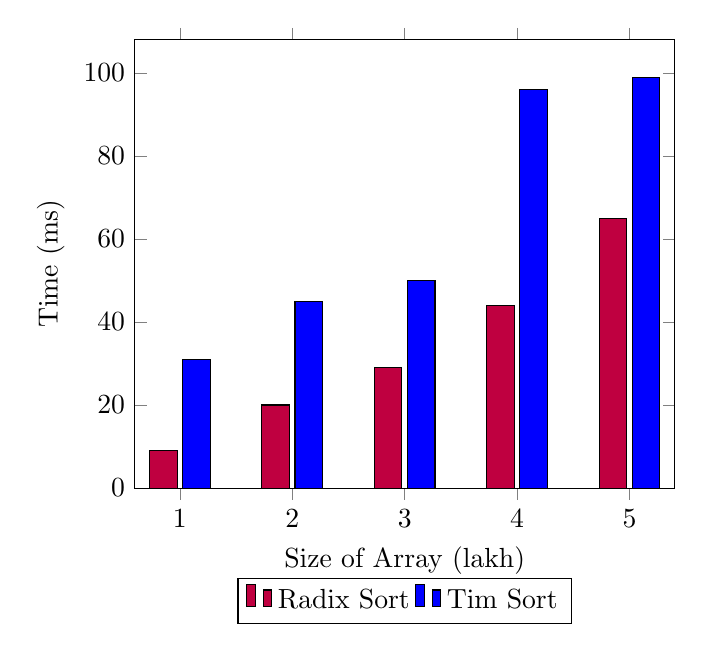
\begin{tikzpicture}
			\begin{axis}[
				ybar,
				bar width=0.35cm,
				xlabel={Size of Array (lakh)},
				ylabel={Time (ms)},
				symbolic x coords={1, 2, 3, 4, 5},
				xtick=data,
				legend style={at={(0.5,-0.2)},
					anchor=north,legend columns=-1},
				]
				\addplot[fill=purple] coordinates {(1, 9) (2, 20) (3, 29) (4, 44) (5, 65)};
				\addplot[fill=blue] coordinates {(1, 31) (2, 45) (3, 50) (4, 96) (5, 99)};
				\legend{Radix Sort, Tim Sort}
			\end{axis}
		\end{tikzpicture}
		\caption{Comparison of Radix Sort and Tim Sort}
		\label{fig:bar-graph}
	\end{figure}
\end{enumerate}
\subsection{Space Complexity Comparison}
\begin{enumerate}
	\item \textbf{Radix Sort : } The space complexity \cite{2} of radix sort is O(n + k), where n is the number of elements and k represents the number of buckets used. It necessitates additional space for creating and managing buckets, which might impact its efficiency in memory-constrained environments.
	\item \textbf{Tim Sort : } Timsort has a space complexity of O(n), requiring additional memory for the merging process and auxiliary arrays. While it also consumes extra space, the amount required is generally proportional to the input size and less than radix sort in typical scenarios.
\end{enumerate}
\subsection{Stability and Adaptability}
\begin{enumerate}
	\item \textbf{Radix Sort : } Radix sort is inherently stable, meaning it preserves the relative order of equal elements. However, its adaptability is limited to scenarios involving fixed-length integer keys or elements with known radix positions.
	\item \textbf{Tim Sort : } Timsort is stable, ensuring the preservation of the original order of equal elements. Its adaptability is notable, especially when handling diverse data distributions or partially ordered sequences, where its adaptive nature shines.
\end{enumerate}
\subsection{Performance on Different Data Distributions}\cite{1}
\begin{enumerate}
	\item \textbf{Radix Sort : } Radix sort performs optimally on fixed-length integer keys, demonstrating efficiency when the number of digits is limited and relatively uniform. However, its performance might degrade with variable-length keys or non-integer data.
	\item \textbf{Tim Sort : } Timsort excels in handling various data distributions, performing well on partially ordered, reverse-ordered, or already sorted data. Its adaptive nature allows it to adjust its performance based on the characteristics of the input sequence.
\end{enumerate}
\section{Conclusion}
Both radix sort  and Timsort offer unique  advantages and are suitable for specific use cases. Radix sort excels in scenarios with fixed-length integer keys, demonstrating linear time complexity but is limited in adaptability to variable-length keys. In contrast, Timsort's adaptability and efficiency across diverse data distributions make it a popular choice for general-purpose sorting tasks, especially when the nature of the data is unpredictable or partially ordered. Choosing between the two algorithms depends on the specific characteristics of the data and the performance requirements of the task at hand.
\section{References}
\bibliography{bib_file.bib}
\bibliographystyle{ieeetr}
\end{document}
